\subsection{HEDM (BraggNN)}
{{\footnotesize
\noindent Uses BraggNN, a deep neural network, for rapid Bragg peak localization in 
high-energy diffraction microscopy, achieving about 13x speedup compared 
to Voigt-based methods while maintaining sub-pixel accuracy.


\begin{description}[labelwidth=4cm, labelsep=1em, leftmargin=4cm, itemsep=0.1em, parsep=0em]
  \item[date:] 2023-10-03
  \item[version:] v1.0
  \item[last\_updated:] 2023-10
  \item[expired:] unknown
  \item[valid:] yes
  \item[valid\_date:] 2023-10-03
  \item[url:] \href{https://arxiv.org/abs/2008.08198}{https://arxiv.org/abs/2008.08198}
  \item[doi:] 10.48550/arXiv.2008.08198
  \item[domain:] Material Science
  \item[focus:] Fast Bragg peak analysis using deep learning in diffraction microscopy
  \item[keywords:]
    - BraggNN
    - diffraction
    - peak finding
    - HEDM
  \item[licensing:] DOE Public Access Plan
  \item[task\_types:]
    - Peak detection
  \item[ai\_capability\_measured:]
    - High-throughput peak localization
  \item[metrics:]
    - Localization accuracy
    - Inference time
  \item[models:]
    - BraggNN
  \item[ml\_motif:]
    - Real-time, Image/CV
  \item[type:] Framework
  \item[ml\_task:]
    - Peak finding
  \item[solutions:] Solution details are described in the referenced paper or repository.
  \item[notes:] Enables real-time HEDM workflows; basis for NAC case study.

  \item[contact.name:] Jason Weitz (UCSD)
  \item[contact.email:] unknown
  \item[results.links.name:] ChatGPT LLM
  \item[fair.reproducible:] True
  \item[fair.benchmark\_ready:] True
  \item[id:] hedm\_braggnn
  \item[Citations:] \cite{liu2021braggnnfastxraybragg}
\end{description}

{\bf Ratings:} ~ \\

\begin{tabular}{p{0.15\textwidth} p{0.07\textwidth} p{0.7\textwidth}}
\hline
Rating & Value & Reason \\
\hline
dataset & 2 & No dataset links or FAIR metadata; unclear public access
 \\
documentation & 3 & Paper is clear, but lacks a GitHub repo or full reproducibility pipeline
 \\
metrics & 4 & Only localization accuracy and inference time mentioned; not formally benchmarked with scripts
 \\
reference\_solution & 3 & BraggNN model is described and evaluated, but no direct implementation or inference scripts available
 \\
software & 2 & No standalone code repository or setup instructions provided
 \\
specification & 5 & None
 \\
\hline
\end{tabular}

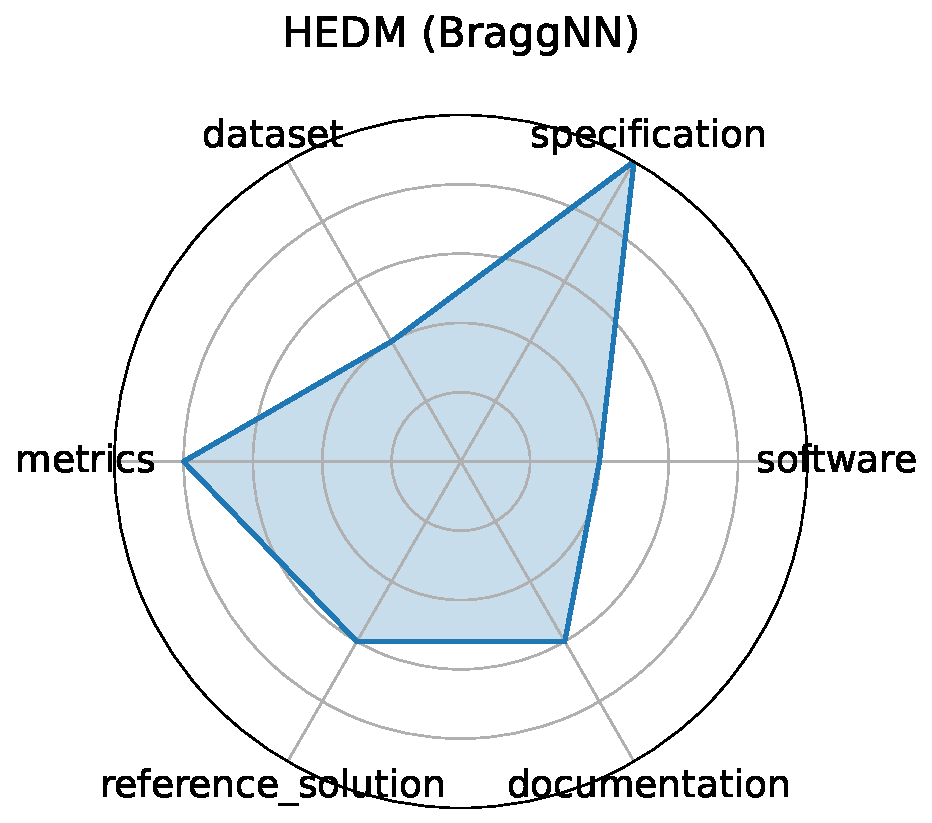
\includegraphics[width=0.2\textwidth]{hedm_braggnn_radar.pdf}
}}
\clearpage